\documentclass[a4paper,12pt]{article}
\usepackage[utf8]{inputenc}
\usepackage{graphicx}
\usepackage{geometry}
\usepackage{titlesec}
\usepackage{fancyhdr}
\usepackage{parskip}
\usepackage{setspace}
\usepackage{enumitem}

\geometry{margin=2.5cm}
\setstretch{1.2}
\pagestyle{fancy}
\fancyhf{}
\rhead{\thepage}
\lhead{Brno University of Technology}

% Title Page
\begin{document}
    \begin{titlepage}
        \centering
        \vspace*{1cm}

        
\includegraphics[width=0.25\textwidth]{template-fig/VUT_symbol_barevne_CMYK_CZ}\par\vspace{1cm} % Replace logo.png with actual filename

        {\Large\textbf{Brno University of Technology}}\\[0.5cm]
        {\large Faculty of Information Technology}\\[2cm]

        {\huge\bfseries Dictionary-Based LZSS Compression with Delta Preprocessing}\\[0.5cm]

        {\large Project Documentation}\\[2cm]

        \begin{flushleft}
            \textbf{Author:} Zdeněk Lapeš\\
            \textbf{Login:} \texttt{xlapes02}\\
            \textbf{Course:} Data Coding and Compression\\
            \textbf{Semester:} Spring 2025
        \end{flushleft}

        \vfill

        {\large \today}

    \end{titlepage}

% Table of contents
    \tableofcontents
    \newpage

% ------------------------------------------------------------------------------

    \section{Introduction}

    This project implements a modular compression and decompression tool based on the LZSS (Lempel–Ziv–Storer–Szymanski) algorithm. The core compression logic follows the traditional LZSS scheme, and the approach presented in this work provides both static and adaptive compression modes. These modes support multiple traversal strategies of the input image, with optional preprocessing using delta encoding.

    The compressor supports command-line usage for compression, decompression, and delta preprocessing of raw
    images. The tool is implemented in C++17.

    The output format is standardized and optionally includes delta-encoded transformations to improve compression efficiency on smoothly varying numeric sequences.

% ------------------------------------------------------------------------------

    \section{Project Goals}
    The goal of this project was to:
    \begin{itemize}
        \item Implement a lossless compression tool using the LZSS algorithm.
        \item Add optional delta preprocessing to improve compression ratio.
        \item Support both static (sequential) and adaptive (block-based) image traversal of raw images that are
        multiples of 16 pixels in width or height.
        \item Provide efficient decompression that restores the original data.
    \end{itemize}

% ------------------------------------------------------------------------------

    \section{Compression Logic}

    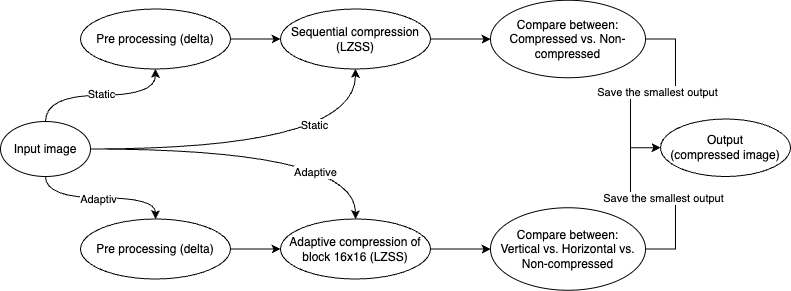
\includegraphics[width=1\textwidth]{template-fig/compressor}\par\vspace{1cm}

    The compression process begins with reading the input image data, optionally applying delta preprocessing, and compressing the result using an LZSS-based method. The goal is to select the most space-efficient output between multiple alternatives.

    \subsection*{Static vs. Adaptive Modes}

    The algorithm supports two main strategies:

    \begin{itemize}
        \item \textbf{Static compression} processes the image sequentially, byte-by-byte, from top to bottom, left to right. This approach is suitable for uniformly structured data.

        \item \textbf{Adaptive compression} divides the image into $16 \times 16$ blocks. Each block is compressed independently, and both horizontal and vertical orientations are evaluated. The orientation yielding the smallest output is selected. This mode requires that both the width and height of the image be divisible by 16.
    \end{itemize}

    In both modes, delta preprocessing can be applied beforehand to transform input into byte differences. This often reveals more redundancy in smooth or gradient-based images.

    \subsection*{Compression Pipeline and Implementation Design}

    The compression pipeline transforms input data into a compact binary format through four main stages, supported by modular components:

    \begin{enumerate}
        \item \textbf{Preprocessing:} When delta encoding is enabled via the \texttt{-m} flag, the input data is
        first transformed by a call to
        \texttt{delta\_encode()} (e.g.\ within \\ \texttt{File::prepare\_adaptive\_blocks\_for\_compression()} for adaptive mode or directly for static mode). The \texttt{File} class is responsible for loading input data, optionally transposing $16\times16$ blocks (if vertical mode is chosen).

        \item \textbf{LZSS Encoding:} The core compression step uses \texttt{Buffer::brute\_force\_search()} to find the longest match between the lookahead buffer and the sliding window, encapsulated in the \texttt{Buffer} structure. This function returns an \texttt{lz\_match} object, containing the offset, length (limited to 31 bytes to fit within 5 bits), and a boolean indicating if a valid match was found. Matches or literal bytes are emitted accordingly within either \texttt{StaticProcessor::compress()} or \texttt{AdaptiveProcessor::compress()}, depending on the compression mode selected.

        \item \textbf{Bit Encoding:} The matches and literals are encoded into a bitstream by the \texttt{BitsetWriter} class. Additionally, a compact 3-byte header—containing metadata like padding size, compression mode, scan direction, delta flag, and image width—is produced by \texttt{BitsetWriter::flush\_to\_file\_after\_compression()}.

        \item \textbf{Comparison and Output Selection:} Specifically for adaptive mode, the algorithm compares
        horizontal and vertical block traversals, selecting whichever yields a smaller bitstream. If the compressed
        size exceeds or equals the original, the \texttt{BitsetWriter} chooses to store the original input
        uncompressed (still with a header for decompression purposes).
    \end{enumerate}

    These components collaborate within the \texttt{StaticProcessor} and \texttt{AdaptiveProcessor} namespaces, depending on the selected mode.

% ------------------------------------------------------------------------------

    \section{Decompression Logic}

    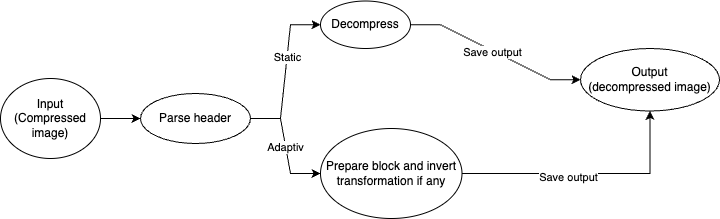
\includegraphics[width=1\textwidth]{template-fig/decompressor}\par\vspace{1cm}

    Decompression reverses the process, reconstructing the original file from the compressed bitstream and metadata.

    \subsection*{Decompression Pipeline}

    The decompression process restores the original data using metadata and the compressed bitstream. The main steps and components are:

    \begin{itemize}
        \item \textbf{Header parsing:} The function \texttt{pre\_decompress(Program\&)} reads the first 3 bytes of the file via \texttt{File::get\_char()} and decodes them into a \texttt{CompressionHeader} struct containing compression mode, scan direction, padding, delta flag, and image width.

        \item \textbf{Bit decoding:} The \texttt{BitsetReader} class extracts literal bytes and \texttt{(offset, length)} matches from the compressed bitstream.

        \item \textbf{Data reconstruction:} Based on the parsed header, either \texttt{StaticProcessor::decompress()} or \texttt{AdaptiveProcessor::decompress()} is invoked to rebuild the data, either sequentially or block-wise with optional transposition.

        \item \textbf{Postprocessing:} If delta encoding was used, the function \texttt{delta\_decode()} restores original byte values by reversing the difference encoding.

        \item \textbf{Output writing:} The \texttt{File} class writes the fully reconstructed data to memory (in \texttt{File::written\_data}) and finally flushes it to the output file.
    \end{itemize}

    This pipeline ensures lossless restoration of the original input, preserving both structure and content across various compression modes.

% ------------------------------------------------------------------------------
    \section{Results}
    {
        \scriptsize
        \begin{tabular}{lrrrrrrr}
            \hline
            Test                               & Original(B) & Compressed(B) & Ratio(\%) & Entropy & OK? & Times(s)        \\
            \hline
            cb.raw (static)                    & 262144      & 20122         & 7.68      & 1.00    & OK  & C:0.039 D:0.010 \\
            cb.raw (static + preprocess)       & 262144      & 20156         & 7.69      & 1.00    & OK  & C:0.038 D:0.014 \\
            cb.raw (adaptive)                  & 262144      & 20122         & 7.68      & 1.00    & OK  & C:0.114 D:0.012 \\
            cb.raw (adaptive + preprocess)     & 262144      & 20125         & 7.68      & 1.00    & OK  & C:0.217 D:0.015 \\
            cb2.raw (static)                   & 262144      & 21099         & 8.05      & 6.91    & OK  & C:0.059 D:0.014 \\
            cb2.raw (static + preprocess)      & 262144      & 22191         & 8.47      & 6.91    & OK  & C:0.107 D:0.011 \\
            cb2.raw (adaptive)                 & 262144      & 21099         & 8.05      & 6.91    & OK  & C:0.317 D:0.013 \\
            cb2.raw (adaptive + preprocess)    & 262144      & 24284         & 9.26      & 6.91    & OK  & C:0.536 D:0.016 \\
            df1h.raw (static)                  & 262144      & 20341         & 7.76      & 8.00    & OK  & C:0.027 D:0.011 \\
            df1h.raw (static + preprocess)     & 262144      & 20099         & 7.67      & 8.00    & OK  & C:0.028 D:0.014 \\
            df1h.raw (adaptive)                & 262144      & 20341         & 7.76      & 8.00    & OK  & C:0.088 D:0.019 \\
            df1h.raw (adaptive + preprocess)   & 262144      & 20099         & 7.67      & 8.00    & OK  & C:0.112 D:0.018 \\
            df1hvx.raw (static)                & 262144      & 23914         & 9.12      & 4.51    & OK  & C:0.195 D:0.017 \\
            df1hvx.raw (static + preprocess)   & 262144      & 22495         & 8.58      & 4.51    & OK  & C:0.263 D:0.014 \\
            df1hvx.raw (adaptive)              & 262144      & 23914         & 9.12      & 4.51    & OK  & C:1.502 D:0.019 \\
            df1hvx.raw (adaptive + preprocess) & 262144      & 23044         & 8.79      & 4.51    & OK  & C:1.577 D:0.026 \\
            df1v.raw (static)                  & 262144      & 25285         & 9.65      & 8.00    & OK  & C:0.344 D:0.024 \\
            df1v.raw (static + preprocess)     & 262144      & 20101         & 7.67      & 8.00    & OK  & C:0.029 D:0.023 \\
            df1v.raw (adaptive)                & 262144      & 25285         & 9.65      & 8.00    & OK  & C:0.724 D:0.021 \\
            df1v.raw (adaptive + preprocess)   & 262144      & 21767         & 8.30      & 8.00    & OK  & C:0.583 D:0.018 \\
            shp.raw (static)                   & 262144      & 20155         & 7.69      & 0.87    & OK  & C:0.037 D:0.014 \\
            shp.raw (static + preprocess)      & 262144      & 20157         & 7.69      & 0.87    & OK  & C:0.032 D:0.031 \\
            shp.raw (adaptive)                 & 262144      & 20108         & 7.67      & 0.87    & OK  & C:0.117 D:0.026 \\
            shp.raw (adaptive + preprocess)    & 262144      & 20103         & 7.67      & 0.87    & OK  & C:0.123 D:0.017 \\
            shp1.raw (static)                  & 262144      & 28786         & 10.98     & 1.90    & OK  & C:0.441 D:0.036 \\
            shp1.raw (static + preprocess)     & 262144      & 29149         & 11.12     & 1.90    & OK  & C:0.442 D:0.021 \\
            shp1.raw (adaptive)                & 262144      & 21311         & 8.13      & 1.90    & OK  & C:0.828 D:0.016 \\
            shp1.raw (adaptive + preprocess)   & 262144      & 21600         & 8.24      & 1.90    & OK  & C:0.805 D:0.016 \\
            shp2.raw (static)                  & 262144      & 37010         & 14.12     & 1.87    & OK  & C:0.736 D:0.013 \\
            shp2.raw (static + preprocess)     & 262144      & 39827         & 15.19     & 1.87    & OK  & C:0.745 D:0.015 \\
            shp2.raw (adaptive)                & 262144      & 28177         & 10.75     & 1.87    & OK  & C:1.300 D:0.019 \\
            shp2.raw (adaptive + preprocess)   & 262144      & 29764         & 11.35     & 1.87    & OK  & C:1.324 D:0.016 \\
            nk01.raw (static)                  & 262144      & 262147        & 100.00    & 6.47    & OK  & C:3.900 D:0.027 \\
            nk01.raw (static + preprocess)     & 262144      & 262147        & 100.00    & 6.47    & OK  & C:3.867 D:0.040 \\
            nk01.raw (adaptive)                & 262144      & 262147        & 100.00    & 6.47    & OK  & C:7.616 D:0.036 \\
            nk01.raw (adaptive + preprocess)   & 262144      & 262147        & 100.00    & 6.47    & OK  & C:7.688 D:0.029 \\
            \hline
        \end{tabular}
    }


% ------------------------------------------------------------------------------

    \section{Testing}

    The project includes a dedicated Python benchmarking script \texttt{benchmarks.py} that automates testing of the
    compression and decompression functionality.

    The script processes benchmark datasets provided in \texttt{tests/in/kko.proj.data}. For each file, it performs:

    \begin{itemize}
        \item Compression in four modes: static, static with delta, adaptive, adaptive with delta.
        \item Decompression and byte-for-byte comparison with the original file to ensure correctness.
        \item Measurement of compression ratios and execution times.
        \item Entropy calculation to evaluate data compressibility.
    \end{itemize}

    All results are printed to stdout in a LaTeX-formatted table, summarizing sizes, ratios, correctness status, time
    measurements, and entropy. This table helps assess not only functional correctness but also performance
    characteristics of each mode.

% ------------------------------------------------------------------------------

    \section{Conclusion}
    The project demonstrates a working implementation of an LZ-based compressor with optional delta encoding and adaptive image traversal. It achieves reasonable compression ratios while maintaining lossless fidelity and supports flexible preprocessing for improved performance on real image data.

    \vfill
    \begin{center}
        \textit{Thank you for reading!}
    \end{center}

\end{document}
